% achemso is the American Chemical Society's class, with the layout of the ACS journals.
% "journal" picks the journal's settings (jacsat = J. Am. Chem. Soc.; others: acsccc,
% jpcafh, orlef7, ...; the full list is in the achemso manual). "manuscript=article" is
% the submission layout: double-spaced, one column, figures where you put them.
% Other values: communication, note, suppinfo (for the Supporting Information file).
% "email=true" prints the corresponding author's address under the affiliations.
\documentclass[journal=jacsat,manuscript=article,email=true]{achemso}

% Chemistry packages: mhchem writes formulae and reactions (\ce{H2O}); siunitx sets
% numbers with units (\qty{25}{\degreeCelsius}) with correct spacing.
\usepackage[version=4]{mhchem}
\usepackage{siunitx}
\usepackage{tikz}
\usepackage{booktabs}

% Authors and affiliations: the class numbers the affiliations with symbols itself. An
% author with several addresses gets \alsoaffiliation; \altaffiliation adds a note such as
% "present address". Give the same \affiliation text to authors who share one.
\author{First Author}
\affiliation[Example University]{Department of Chemistry, Example University, City, Country}
\author{Second Author}
\altaffiliation{These authors contributed equally.}
\affiliation[Example University]{Department of Chemistry, Example University, City, Country}
\author{Corresponding Author}
\email{corresponding.author@example.edu}
\phone{+00 000 000 0000}
\affiliation[Example Institute]{Institute of Chemical Research, City, Country}
\alsoaffiliation[Another University]{Department of Physical Chemistry, Another University, City, Country}

\title{A Specific Title that Names the System and the Finding: Keep It Under Two Lines}


\begin{document}

% The abstract of an ACS manuscript is one paragraph of at most 250 words: the problem,
% the key result with a number, and why it matters.
\begin{abstract}
Summarise what was made or measured, how, and what the main result is, for example a
yield, a rate constant or a binding energy. Formulae can be written with mhchem, as in
the oxidation of \ce{CO} to \ce{CO2} over a \ce{Pt}/\ce{Al2O3} catalyst with a turnover
frequency of \qty{12}{\per\second}.
\end{abstract}

% The Table of Contents graphic is required by ACS journals. It sits in its own
% environment (printed on a page of its own, after the references) and must be at most
% 3.25 in x 1.75 in (8.25 cm x 4.45 cm). Replace the drawing by \includegraphics{toc.png}:
% a single image, no caption, ideally with no more than a short text.
\begin{tocentry}
  \begin{tikzpicture}
    \draw[gray] (0.05,0.05) rectangle (8.2,4.4);
    \node[gray,align=center] at (4.125,2.225) {TOC graphic placeholder\\8.25 cm $\times$ 4.45 cm};
  \end{tikzpicture}
\end{tocentry}

\maketitle

\section{Introduction}
State the problem and what is known, citing earlier work\cite{pauling31,woodward65}.
References are numbered as superscripts after the punctuation, the ACS style;
\verb|\citenum| names a reference in running text, as in Ref.~\citenum{atkins10}. Close the
section with one sentence on what this paper adds.

\section{Results and Discussion}
Reactions and formulae go in \verb|\ce|: \ce{2 H2 + O2 -> 2 H2O}. Charges, states and
reaction arrows work too:
\begin{equation}
  \ce{[Fe(H2O)6]^{3+} + SCN- <=> [Fe(SCN)(H2O)5]^{2+} + H2O}
  \label{eq:equilibrium}
\end{equation}
Equation~\ref{eq:equilibrium} has the equilibrium constant $K = \qty{1.4e2}{\litre\per\mole}$ at
\qty{25}{\degreeCelsius}; \verb|\qty| puts a thin space before the unit, and
\verb|\SI| from older siunitx works as well. In ACS papers equations are numbered
only when you refer to them.

Table~\ref{tab:kinetics} shows how a table looks: ACS tables have a caption above and
no vertical rules.

\begin{table}
  \caption{Rate constants for the reaction at \qty{298}{\kelvin}}
  \label{tab:kinetics}
  \begin{tabular}{lcc}
    \toprule
    Catalyst & $k$ (\unit{\per\second}) & Yield (\%) \\
    \midrule
    \ce{Pt/Al2O3} & \num{1.2e-2} & 94 \\
    \ce{Pd/C}     & \num{3.4e-3} & 81 \\
    \bottomrule
  \end{tabular}
\end{table}

\begin{figure}
  \centering
  % A reaction scheme or plot goes here: \includegraphics[width=\linewidth]{scheme.pdf}
  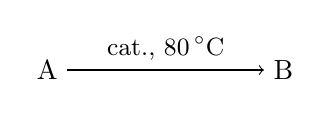
\begin{tikzpicture}[x=1cm,y=1cm]
    \node (a) at (0,0) {\ce{A}};
    \node (b) at (3,0) {\ce{B}};
    \draw[->] (a) -- node[above] {\small cat., \qty{80}{\degreeCelsius}} (b);
  \end{tikzpicture}
  \caption{Captions go under figures and schemes and say what the reader sees.}
  \label{fig:scheme}
\end{figure}

\section{Conclusions}
Two or three sentences: what was shown, and the most useful next experiment.

\section{Experimental Section}
\subsection{General Methods}
Say where reagents came from, and how solvents were dried. Report amounts as
\qty{5.0}{\milli\mole} and \qty{10}{\milli\litre}, and spectra as
$^{1}$H~NMR (\qty{400}{\mega\hertz}, \ce{CDCl3}) $\delta$~7.26.

\begin{acknowledgement}
Thank funding bodies and colleagues here; ACS journals print this as an unnumbered
section before the references.
\end{acknowledgement}

% The class prints the heading "Supporting Information Available"; you write the note.
% The Supporting Information itself is a separate file (use manuscript=suppinfo for it).
\begin{suppinfo}
Experimental procedures, characterisation data,
NMR spectra and computational details are available free of charge.
\end{suppinfo}

\bibliography{refs}

\end{document}
